%!TEX root=paper.tex

% \newpage
\section{How Do Students Use the Possibility of Reading Personally Interesting Articles?}
\label{sec:results}


% \subsection {Feed Subscriptions}
Figure \ref{fig:subscriptions} represents an incidence matrix collected at the end of the study interval: the columns represent students, and the rows represent article sources; if a student is registered to a given source, at the intersection of the corresponding row and column we place a $\Diamond$. 

We would expect to see fully continuous horizontal rows of data-points if every user subscribed to the same feed, and fully continuous vertical rows if every user subscribed to all of the feeds available. The fact that these patterns are largely absent in Figure \ref{fig:subscriptions} supports our assumption that different individuals prefer to subscribe to different reading sources.

% The figure illustrates that giving the students the freedom to choose the sources they wanted, allowed each one of them to express their interest. 

\begin{figure}[h!]

\centering
  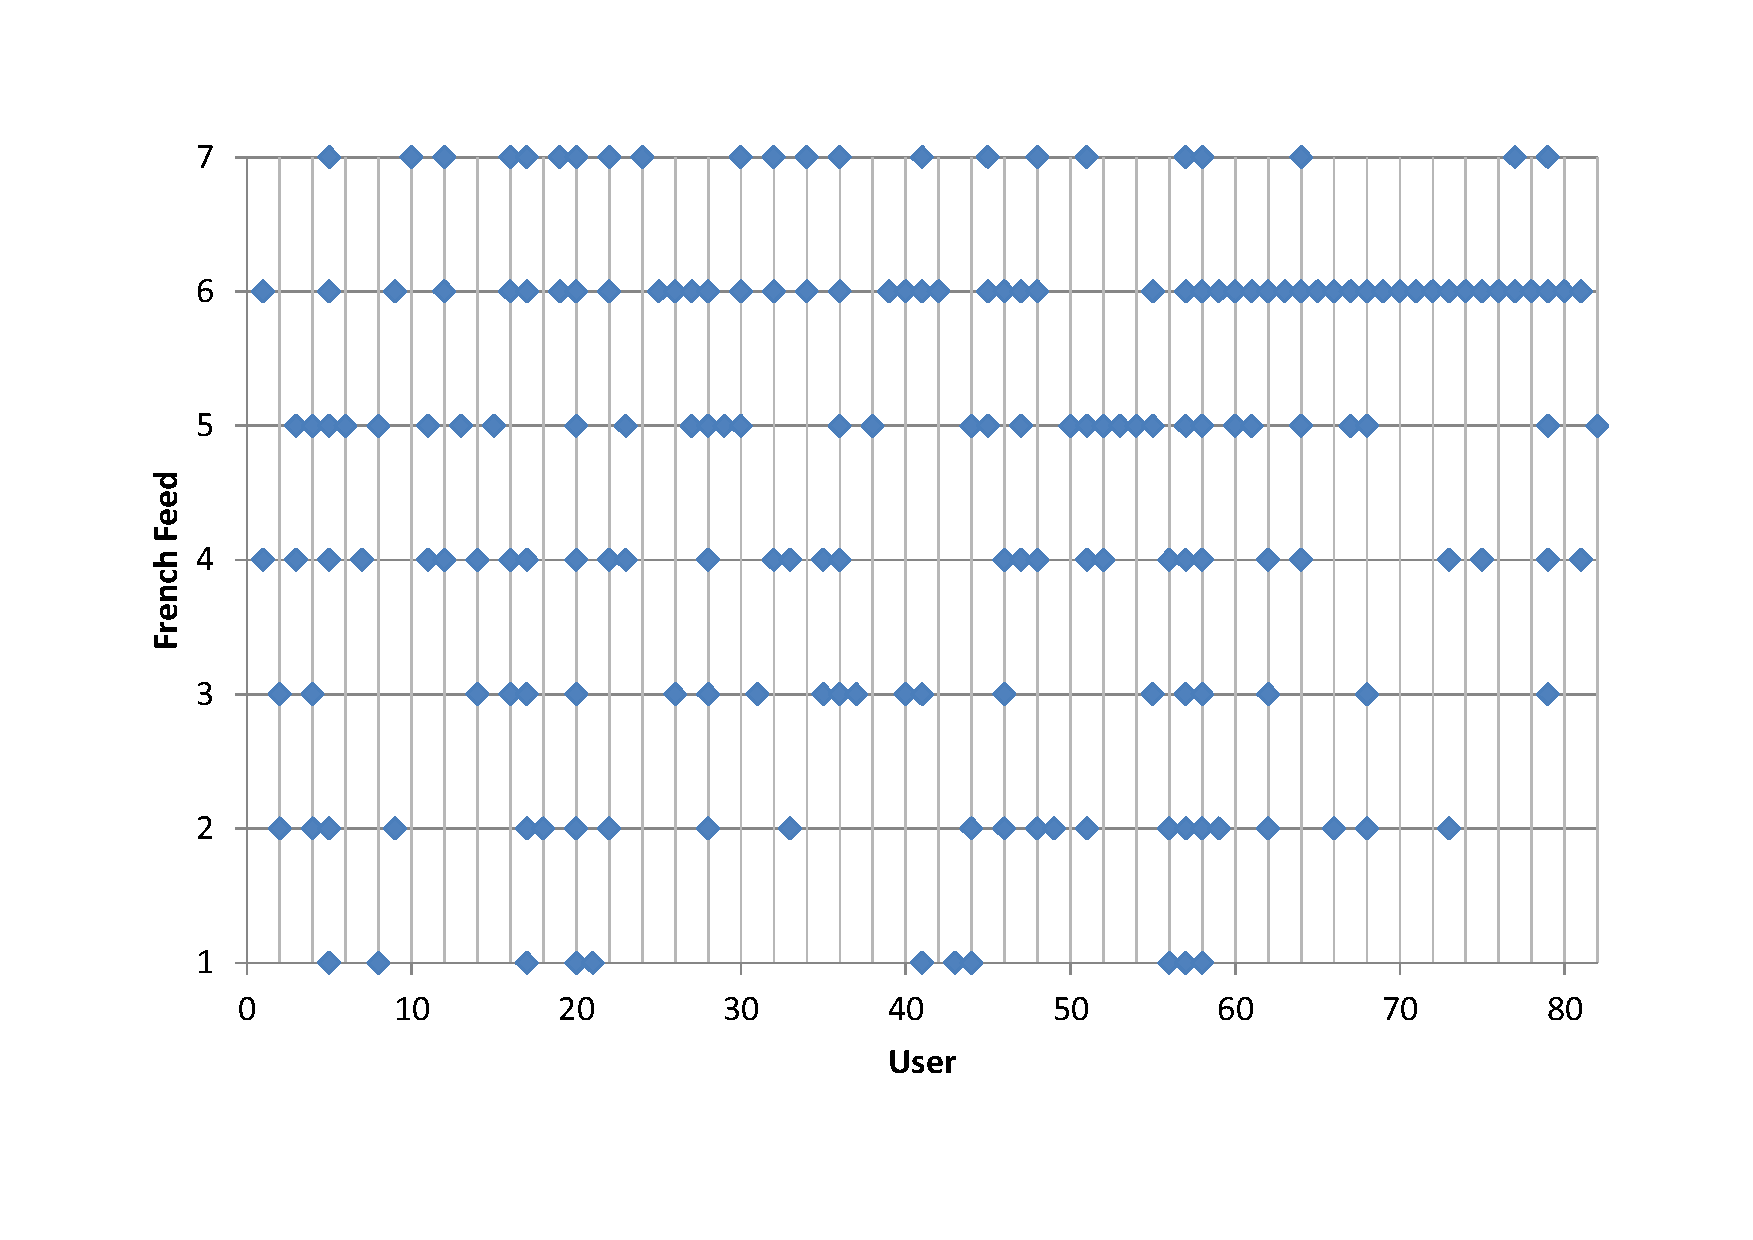
\includegraphics[width=\columnwidth]{figures/users_feeds}
  \caption{Different users subscribe to different sources}
  \label{fig:subscriptions}  
\end{figure}

Of course some feeds are more popular than others. Projecting the data- points onto the horizontal axis and sorting the results leaves us with a histogram as can be seen in Figure \ref{fig:feedpopularity}.

\begin{figure}[h!]
\centering
  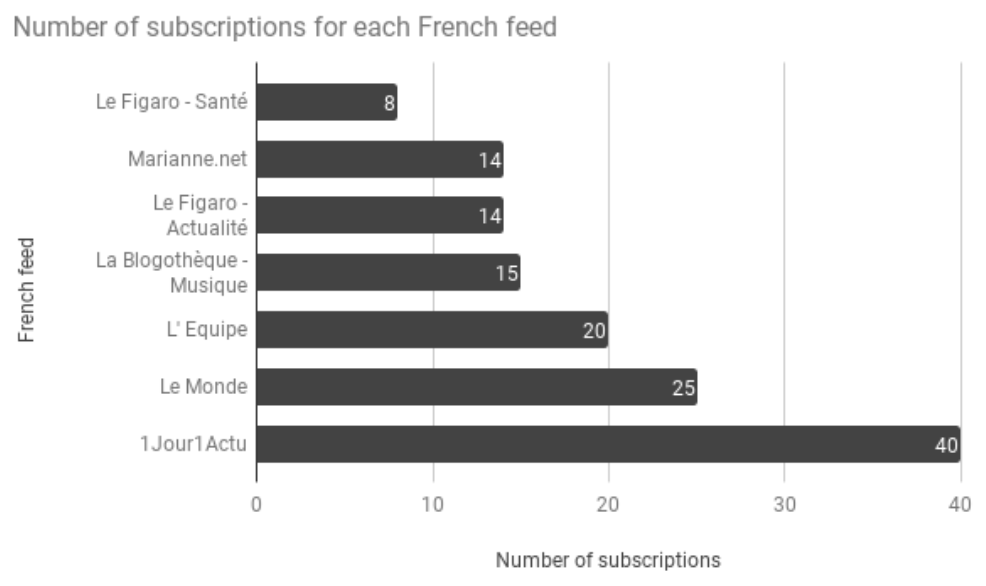
\includegraphics[width=\columnwidth]{figures/feed_popularity}
  \caption{Some feeds are more popular than others}
  \label{fig:feedpopularity}
\end{figure}


{\em 1Jour1Actu} is the most popular article source and Le Figaro - Sant\'e is the least. In order to see whether or not this might be related to how they are presented in the dialog window of our system (see Figure \ref{fig:system_subscriptions}), in Figure \ref{fig:popularityvsranking} can compare the order of popularity with the order in which they are displayed. One can see how the second-to-last presented feed, Le Monde, is the second most popular feed by measure of subscriptions. Conversely, the feed listed above Le Monde is actually the least subscribed-to feed in our listing.


\begin{figure}[h!]
\centering
  \newcommand{\picscale}{0.5}
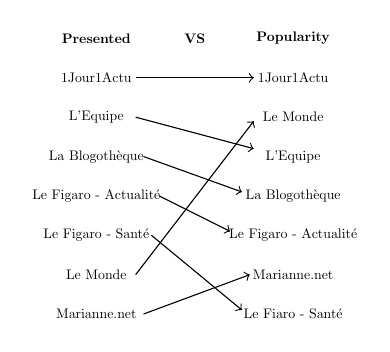
\begin{tikzpicture}[scale=\picscale, every node/.style={scale=\picscale}]
    % Columns.
    \node at (0  , 0) {\bf Presented};
    \node at (2.5, 0) {\bf VS};
    \node at (5  , 0) {\bf Popularity};
    
    % As presented.
    \node at (0,-1) {1Jour1Actu};
    \node at (0,-2) {L'Equipe};
    \node at (0,-3) {La Blogoth\`{e}que};
    \node at (0,-4) {Le Figaro - Actualit\'{e}};
    \node at (0,-5) {Le Figaro - Sant\'{e}};
    \node at (0,-6) {Le Monde};
    \node at (0,-7) {Marianne.net};
    
    % As popular.
    \node at (5,-1) {1Jour1Actu};
    \node at (5,-2) {Le Monde};
    \node at (5,-3) {L'Equipe};
    \node at (5,-4) {La Blogoth\`{e}que};
    \node at (5,-5) {Le Figaro - Actualit\'{e}};
    \node at (5,-6) {Marianne.net};
    \node at (5,-7) {Le Fiaro - Sant\'{e}};
    
    % Arrows between presented and popular.
    \draw [->] (1,-1)   --   (4,-1);
    \draw [->] (1,-2)   --   (4,-2.8);
    \draw [->] (1.2,-3) --   (3.7,-3.9);
    \draw [->] (1.6,-4) --   (3.4,-4.9);
    \draw [->] (1.4,-5) --   (3.7,-6.9);
    \draw [->] (1,-6)   --   (4,-2.1);
    \draw [->] (1.2,-7) --   (3.9,-6);
    
\end{tikzpicture} 
  \caption{The popularity of the feeds vs. their ranking in the UI}
  \label{fig:popularityvsranking}
\end{figure}




\subsection{Article Interactions}
Figure \ref{fig:articles_read} shows that the articles that the users interact with present a similar pattern: each user explores their own interest, and there is no one article that is interesting for all. The vertical ``line '' in the figure represents an over-active reader.

\begin{added}

  Interacting with means that the user translated at least one word in that article. to check with Dan that this is the definition! we currently do not have information about whether a user read the article to the end. 

\end{added}

\begin{figure}[h!]
\centering
  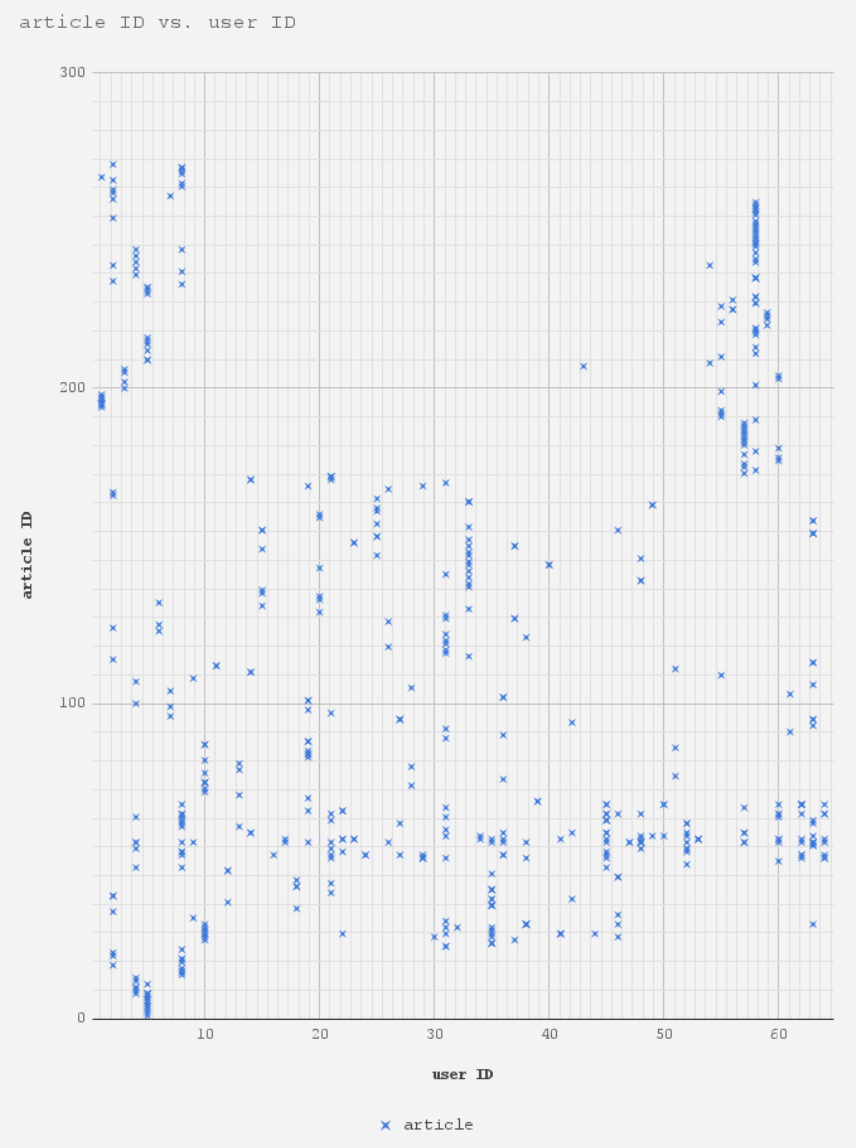
\includegraphics[width=0.9\columnwidth]{figures/users_articles}
  \caption{Every student has their own article reading preferences}~\label{fig:articles_read}
\end{figure}

\begin{added}

  After investigating some of the patterns of reading of students we observed that there are those who enjoy reading a variety of topics, but also those who like to read a single topic. 
  From the latter category student \#608 has read twelve articles exclusively on topics about sports in five different days and student \#617 has read 6 articles exclusively about health topics over two distinct days.
    % The student \#657 in the published dataset has read 10 articles exclusively about sport in three different days between June 7 and July 4th. 
  
\end{added}

\section{How Are The Reader Features Used?}
\newcommand{\feature}[1]{{\em #1}}
Given that the reader interaction more innovative and more complex than the one to be found in exercises, we decide to use telemetry to investigate how are the learners using these features. Telemetry has been successfully used for understanding user behavior in games \cite{Gagne11-telemetry} but also more generic contexts, such as automatically detecting personas from large scale interaction data \cite{Zhang16-telemetry}. In our study, we used telemetry to track the usage of various relevant features in the personalized textbook in order to better understand the usage of our system.

Based on logging every interaction of every user, Figure \ref{fig:feature_usage} shows the six most used features of the system.\footnote{An extended analysis that includes more features is presented elsewhere. \cite{Chirtoaca17-apollo}}

  \begin{figure}[h!]
  \centering
    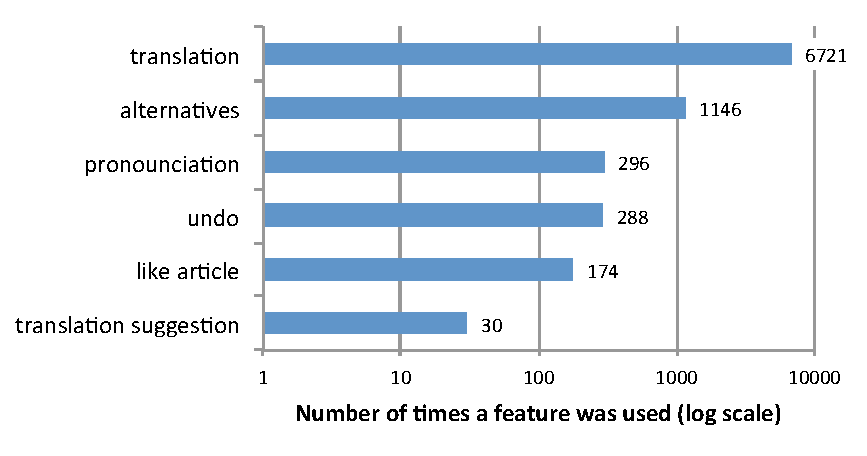
\includegraphics[width=0.9\columnwidth]{figures/reader_feature_usage}
    \caption{Popularity of features by their recorded usage-events}
    \label{fig:feature_usage}
  \end{figure}

With 6.700 occurrences, \feature{requesting a translation for a word} is the most used interactive feature of the system. The second most used feature is \feature{opening the translation alternatives} drop-down list. The six-to-one ration between the two features is an indicator of the limitations of the automatic translation -- it seems that one in six translations are not satisfying to the learners.

The third most used feature is \feature{pronunciation}. On average, there are about 1.66 pronunciations for a given translation, suggesting that users are often asking for a second pronunciation after hearing it the first time. 

% \ml{@dan, do you agree with this conclusion? it's opposite to your thesis, but I think this is the correct interpretation}

% In addition, we looked at the number of times the same word or phrase was pronounced by the same user. This data ranges from one single pronunciation to 14 pronunciations for the same word (phrase). The size of this interval is mostly due to the users' different proficiency in a certain language and the difficulty in pronunciation of the word (phrase) itself. Nevertheless, on average, the number approaches 1.66 pronunciation requests for the same piece of text, suggesting that users are generally sufficiently content with a pronunciation after hearing it the first time.


\feature{Undo}-ing a translation is used when the user wants to remove the last translation that was inserted in the text. For the proposed interaction mechanism this feature seems to be useful. 

A {\em like} button found at the bottom of an article  was clicked by the readers 174 times. Although not used at the moment, this information can be used in the future to improve article recommendations.
 % and maybe to add a social dimension to the system by providing information about how other people react to a given article.

The least used feature presented in the Figure \ref{fig:feature_usage}, {\em translation suggestion}, allows users to contribute their own translations when they are not satisfied with the one automatically provided by the system. 
% \ml{which brings me to: @Dan, what do you mean by alternatives here? :) Is it the number of times somebody selected an alternative, or the number of times they opened the menu. In any case, can we get the other number?}

  \begin{figure}[h!]
  \centering
    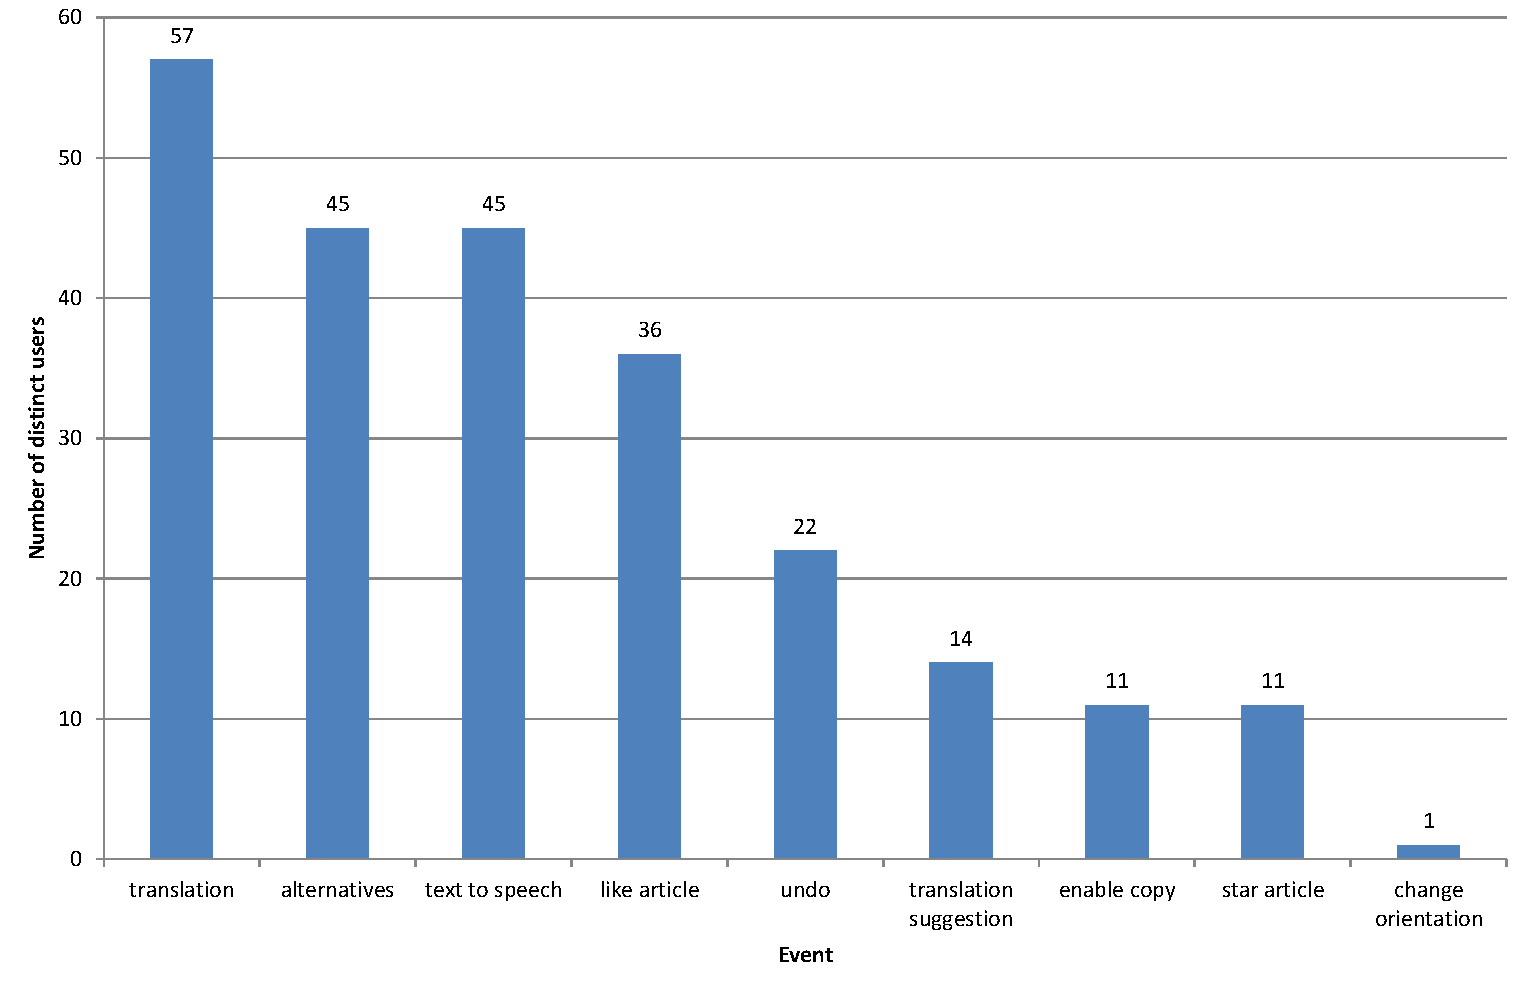
\includegraphics[width=0.9\columnwidth]{figures/reader_feature_usage_per_user}
    \caption{The usage of the various reader features by the various users }
    \label{fig:usage_per_user}
  \end{figure}


Figure \ref{fig:usage_per_user} shows the number of distinct users for each category of events. A larger number of distinct users indicates a feature that is more important to the students. We see that: 
\begin{itemize}
  \item Not all the users of the system use translations
  \item \feature{Translation suggestion} is used by very few users. It still is to be determined whether this is due to readers overwhelmingly being satisfied with the automatic translations and their alternatives, or due to a low involvement. 
\end{itemize}



\newpage
\section{How Do Students Use the Personalized Vocabulary Exercises?}

The system presented four types of vocabulary practice exercises to the students. In total, during the entire duration of the study we observed 18.082 exercises being presented to the students. Figure \ref{fig:ex_interactions} presents the number of exercises which had a ``correct'' outcome (red) vs. exercises which had a ``wrong'' outcome (blue). The figure shows one student who did 3.000 (!) exercises during one month, and about six eager students who did more than 700 exercises. 

  \begin{figure}[h!]
  \centering
    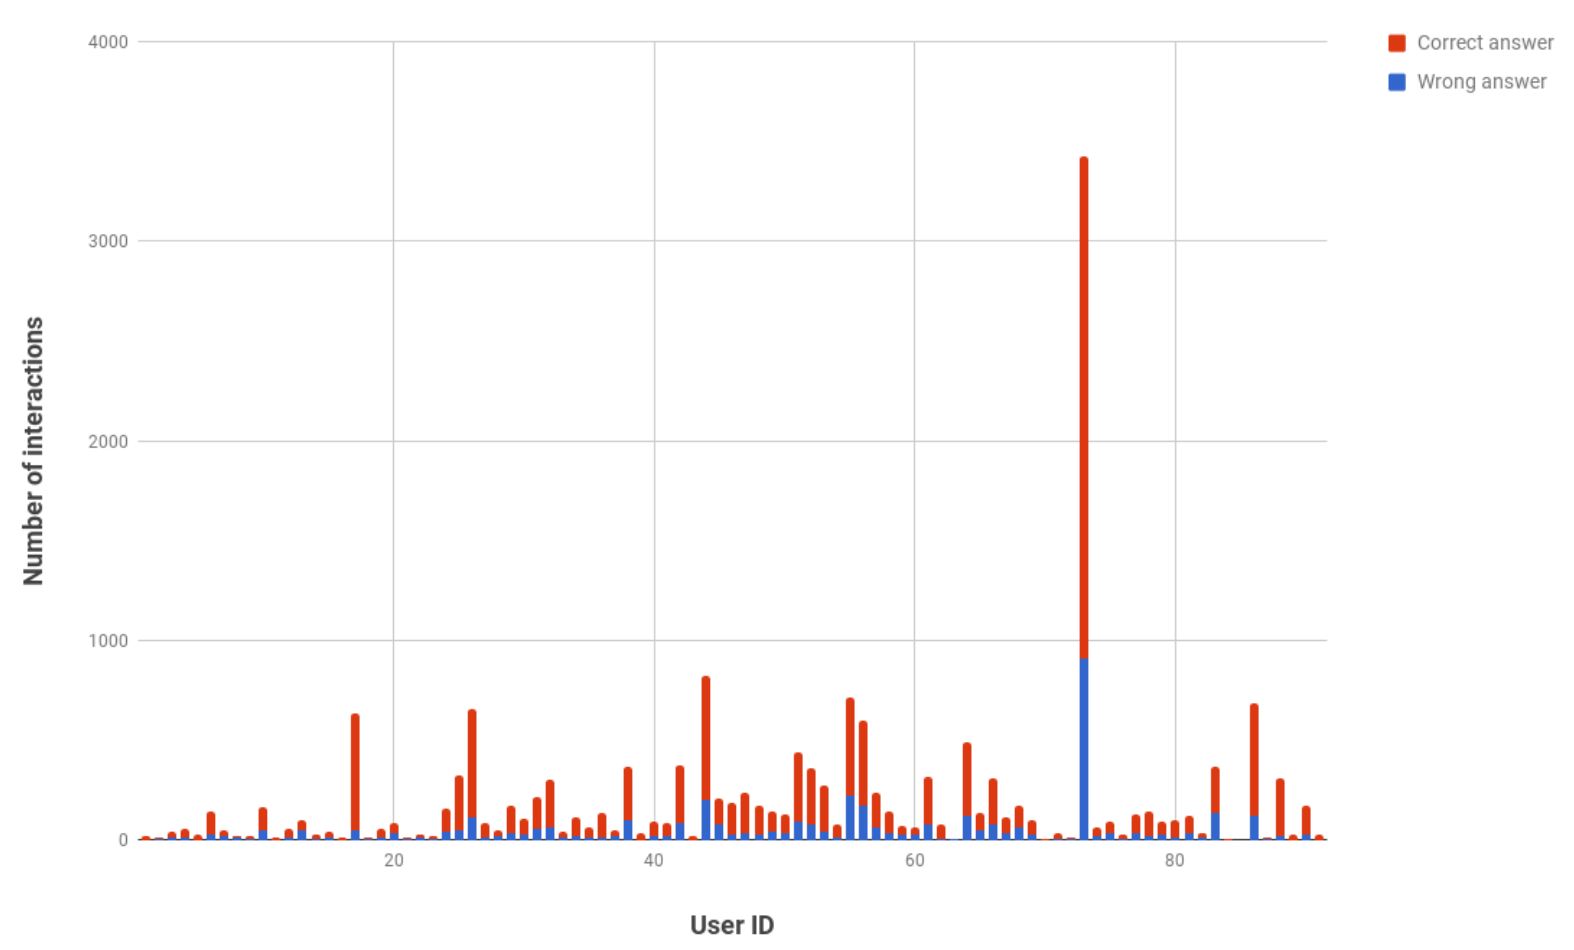
\includegraphics[width=\columnwidth]{figures/exercise_interactions_count.png}
    \caption{Correct (red) and wrong (blue) exercise outcomes per student}
    \label{fig:ex_interactions}
  \end{figure}

The figure does not include one other type of outcome, {\em requesting a hint}, which is presented in the table below grouped per exercise type. The corresponding number of hints suggests that the multiple-choice exercises (i.e. Match, Choose) are simpler than free text entry exercises (i.e. Find, Translate).

\begin{tabular}{lrrrr}
  % source id: 
  % choose -- 5
  % find -- 4
  % translate -- 7
  % match -- 6
                      & Choose  & Find & Translate & Match \\ \hline
  Total interactions  & 7180    & 6249 & 2643      & 2010\\
  Hint requests       & 29      & 529  & 847       & 16 \\ \hline
  \label{tab:hints_per_ex_type}
\end{tabular}

Figure \ref{fig:activity_per_day} shows the days when learners practice exercises. It suggests constant activity over the entire period of the study with a more intensive period towards the end.

  \begin{figure}[h!]
  \centering
    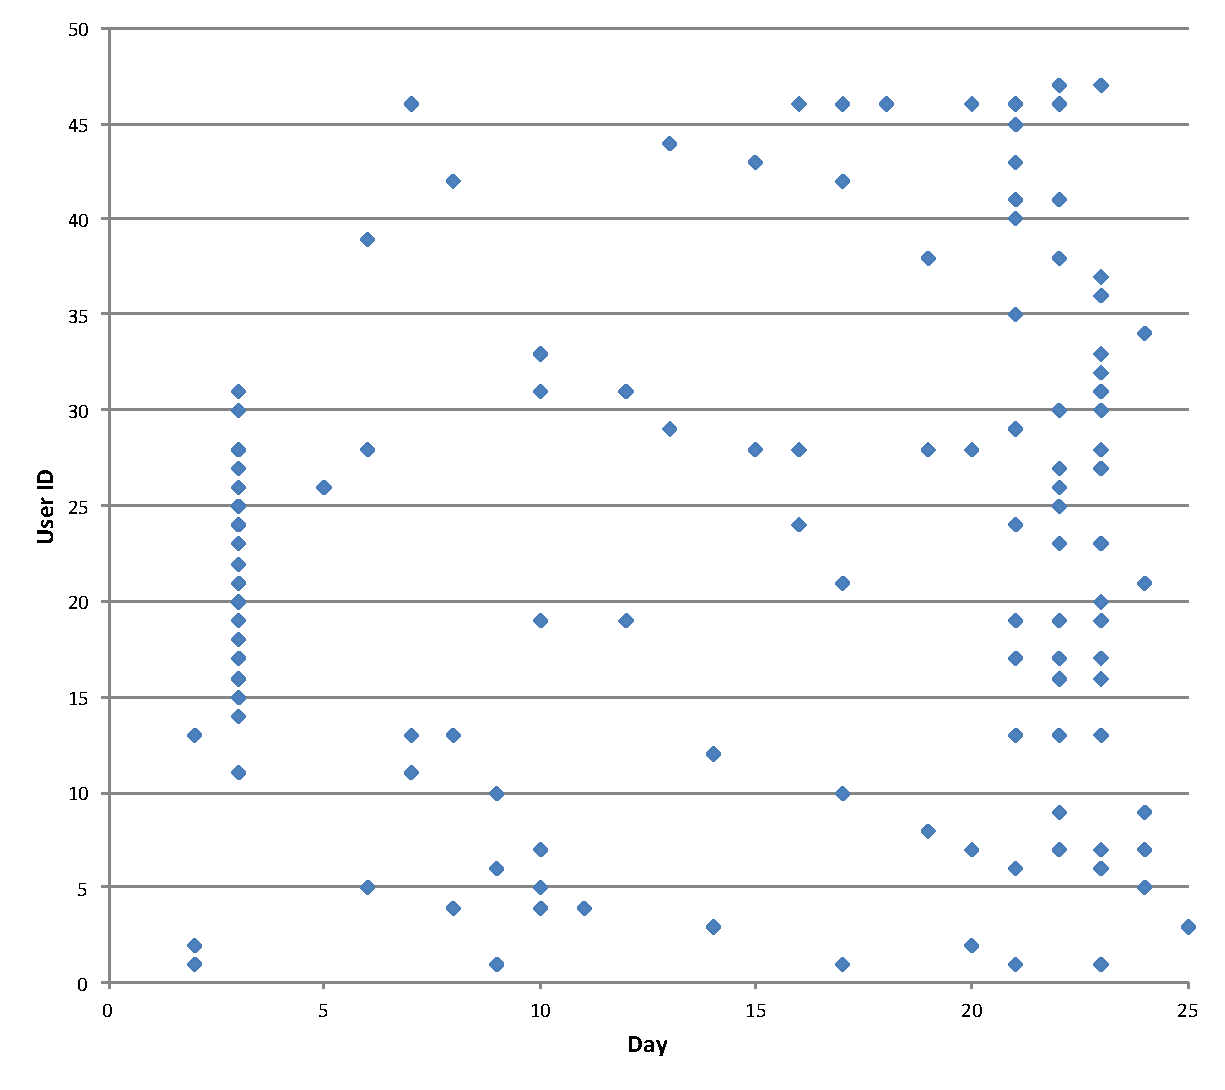
\includegraphics[width=0.8\columnwidth]{figures/user_exercise_activity_vs_day.pdf}
    \caption{The students are doing exercises at their own pace throughout the one month interval }
    \label{fig:activity_per_day}
  \end{figure}


\begin{added}


\section{Do Students Improve Their Vocabulary?}
\section{How Does The System Help Students Improve Their Vocabulary?}

  The value of extensive reading and vocabulary practice can be found, besides the new words that are learned, also in the strengthening of the knowledge of the existing words. This is hard to quantify, but by analyzing the learner interaction with the exercises we can provide a glimpse into it. Looking at the outcomes of all the exercises done by the students we observe that:

  \begin{itemize}
    \item In total 5149 words were used in the exercises platform during the learning period. They are words for which the learners requested a translation before. Therefore the learners either did not know them or at least were unsure about them.

    \item For 80\% (4110) of the words the learners were able to correctly identify the meaning in the last associated exercise. Out of these: 

    \begin{itemize}
      \item 14\% were wrong during their first interaction in exercises but were correct in the final iteration of the exercises. These are {\bf likely to be learned via the exercises}.

      \item 66\% were recognized already for the first time in the exercises. These are {\bf likely to be words for which the knowledge was strengthened by using the system}: the students were unsure when encountering them initially in texts but eventually knew their meaning when encountering them later in the exercises. 
    \end{itemize}

    \item For 20\% (1037) of the words the final outcomes showed incorrect answers, thus we can assume that they remained {\bf unlearned at the end of the experimental period}.

  \end{itemize}

\end{added}









